\section{测度空间}
\label{sec:measure-spaces-def}

上一节提出的两项要求分别针对不同对象：一项限定哪些集合允许测量，另一项规定怎样给这些集合赋予大小。本节把它们分开建立。先用$\sigma$代数描述允许测量的集合族，在度量空间上由开集得到Borel集；再在其上定义可数可加的测度，推出比较、取极限与加权的规则；最后讨论哪些例外可以忽略，以及怎样把零测集的子集纳入可测范围。

\subsection{$\sigma$代数}
\label{sec:measure-sigma-algebras}

\paragraph{能够区分哪些集合}
设$X=\{1,2,3,4\}$。若允许测量全部$16$个子集，就能单独询问每个点的大小；若只知道每个点属于$\{1,2\}$还是$\{3,4\}$，能够回答的只有$\varnothing$、$\{1,2\}$、$\{3,4\}$、$X$这四个集合是否发生，单点$\{1\}$无法单独测量。两种集合族底集相同，区分能力不同。无论选哪一种，只要$A$允许测量，“不在$A$中”也应允许测量；只要一列集合都允许测量，“至少属于其中一个”也应允许测量。这正是上一节对可数运算的要求。

\begin{definition}[$\sigma$代数]
\label{def:measure-sigma-algebra}
设$X$是集合，$\mathcal A$是$X$的一族子集。若
\begin{enumerate}
 \item $X\in\mathcal A$；
 \item $A\in\mathcal A$蕴含$X\setminus A\in\mathcal A$；
 \item $A_1,A_2,\dots\in\mathcal A$蕴含$\bigcup_{n\ge1}A_n\in\mathcal A$，
\end{enumerate}
则称$\mathcal A$为$X$上的一个\term{$\sigma$代数}（sigma-algebra），称$(X,\mathcal A)$为\term{可测空间}（measurable space），称$\mathcal A$中的集合为\term{可测集合}（measurable set）。
\end{definition}

定义只列出补集与可数并，其他运算由它们得到。由第1、2条，$\varnothing=X\setminus X\in\mathcal A$；在第3条中从某项起全取$\varnothing$，得到有限并封闭。可数交由De Morgan律化为补集与并：
\[
 \bigcap_{n\ge1}A_n=X\setminus\bigcup_{n\ge1}(X\setminus A_n),
\]
差集$A\setminus B=A\cap(X\setminus B)$也属于$\mathcal A$。所以从可测集合出发，经可数次补、并、交、差得到的集合仍然可测。开头的两种集合族都满足这些条件：幂集$\mathcal P(X)$含全部子集，任何运算结果都仍在其中；四个集合$\{\varnothing,\{1,2\},\{3,4\},X\}$中任一个的补集仍在其中，任意几个的并也在其中。

\paragraph{生成的$\sigma$代数}
实际问题中我们通常只点名少数必须能测量的集合，例如区间或若干类别，希望由它们补齐其余集合。给定$X$的一族子集$\mathcal C$，包含$\mathcal C$的$\sigma$代数至少有幂集一个。令$\sigma(\mathcal C)$为所有包含$\mathcal C$的$\sigma$代数之交，称为$\mathcal C$\term{生成的$\sigma$代数}（generated sigma-algebra）。逐条核对：每个参与求交的$\sigma$代数都含$X$，对补集、可数并封闭，交集中的元素同时属于它们全体，运算结果也同时属于它们全体，所以$\sigma(\mathcal C)$是$\sigma$代数；它包含$\mathcal C$，又包含于任何包含$\mathcal C$的$\sigma$代数，因此是其中最小的一个。

\begin{example}[有限分组生成的$\sigma$代数]
\label{ex:measure-partition-sigma}
在$X=\{1,2,3,4\}$上取$\mathcal C=\{\{1\},\{2\}\}$。生成的$\sigma$代数必须含$\{1\}$、$\{2\}$以及$X\setminus(\{1\}\cup\{2\})=\{3,4\}$，于是含有分组$\{1\},\{2\},\{3,4\}$中任意几组的并，共$2^3=8$个集合。这$8$个集合对补集和并已经封闭，所以它们就是$\sigma(\mathcal C)$；$\{3\}$不在其中。一般地，有限集合被分成$k$组时，由各组生成的$\sigma$代数恰由若干组之并组成，共$2^k$个集合。图~\ref{fig:measure-partition-sigma}比较了三种分组：组分得越细，可以单独测量的集合越多。
\end{example}

\begin{figure}[!htbp]
  \centering
  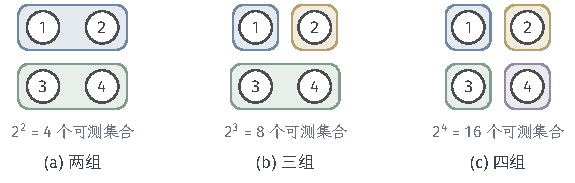
\includegraphics[width=97.3mm]{figures/02-abstract-mathematics/01-metric-and-measure/tikz/c2-sigma-algebra-partition/figure.pdf}
  \caption{四点集合$X=\{1,2,3,4\}$上由分组生成的$\sigma$代数。每个色块是一组，可测集合恰是若干组之并。(a)分成$\{1,2\},\{3,4\}$两组，得到$2^2=4$个可测集合；(b)分成$\{1\},\{2\},\{3,4\}$三组，得到$2^3=8$个；(c)每点自成一组，得到全部$2^4=16$个子集。}
  \label{fig:measure-partition-sigma}
\end{figure}

生成操作补齐的只是可数运算的封闭性，未必得到所有希望测量的集合。在$\mathbb R$上取全体单点组成的族$\mathcal C$。令$\mathcal D$为$\mathbb R$中可数集合与补集可数的集合的全体：它含$\mathbb R$；可数集的补集补集可数，反之亦然；一列集合若都可数，并可数，若有一个补集可数，并的补集包含于它的补集，也可数。所以$\mathcal D$是含全部单点的$\sigma$代数，$\sigma(\mathcal C)\subseteq\mathcal D$。而$[0,1]$与它的补集都不可数，$[0,1]\notin\mathcal D$。因此单点生成的$\sigma$代数不含任何区间，要测量区间，生成族里必须直接放入区间或开集。

\paragraph{迹$\sigma$代数与子$\sigma$代数}
改变“可测范围”有两种不同的操作。第一种缩小底集：设$Y\subseteq X$，令$\mathcal A_Y=\{A\cap Y:A\in\mathcal A\}$。由$(A\cap Y)$在$Y$中的补集为$(X\setminus A)\cap Y$，以及$\bigcup_n(A_n\cap Y)=(\bigcup_nA_n)\cap Y$，它是$Y$上的$\sigma$代数，称为\term{迹$\sigma$代数}（trace sigma-algebra）。第二种保持底集不变、只保留一部分可测集合：若$\mathcal G\subseteq\mathcal A$本身也是$X$上的$\sigma$代数，称$\mathcal G$为$\mathcal A$的\term{子$\sigma$代数}（sub-sigma-algebra）。

仍取$X=\{1,2,3,4\}$与$\mathcal A=\mathcal P(X)$。迹$\sigma$代数$\mathcal A_{\{1,2\}}=\mathcal P(\{1,2\})$丢掉了点$3,4$，剩下的点仍可逐个区分；子$\sigma$代数$\mathcal G=\{\varnothing,\{1,2\},\{3,4\},X\}$保留全部四个点，却只能分辨它们属于哪一组。前者改变研究对象，后者改变对同一批对象的分辨精度。后面讨论“只掌握部分信息”时，所用的正是子$\sigma$代数。

\subsection{Borel $\sigma$代数}
\label{sec:measure-borel-sets}

\paragraph{由开集生成}
在度量空间中已经有一族自然的集合：开集。第~\ref{sec:metric-open-closed}节用开球定义了开集与闭集，连续性、收敛与紧性都通过它们表达。把开集作为生成族，就得到与这些结构相容的可测范围。

\begin{definition}[Borel $\sigma$代数]
\label{def:measure-borel}
设$(X,d)$是度量空间。由全体开集生成的$\sigma$代数称为$X$的\term{Borel $\sigma$代数}（Borel sigma-algebra），记作$\mathcal B(X)$，其中的集合称为\term{Borel集}（Borel set）。
\end{definition}

开集的补集是闭集，所以闭集都是Borel集；可数个闭集的并、可数个开集的交也是Borel集。例如$\mathbb Q$是可数个闭集$\{q\}$的并，$[0,1)=\bigcap_{n\ge1}(-1/n,1)$是可数个开集的交，二者都是Borel集。需要强调，$\mathcal B(X)$只规定了哪些集合允许测量，并没有规定任何集合的大小；同一个Borel结构上可以放置长度、点质量或它们的组合等不同测度。

\paragraph{实轴上的生成族}
在$\mathbb R$上直接处理全部开集并不方便，下面说明较小的区间族已经足够。关键是把任意开集写成可数个区间的并。

\begin{lemma}[开集的有理区间表示]
\label{lem:measure-open-rational-intervals}
$\mathbb R$中每个开集$U$都是有理端点开区间的可数并。
\end{lemma}

\begin{proof}
任取$x\in U$。由$U$是开集，存在$r>0$使$(x-r,x+r)\subseteq U$。有理数在实轴上稠密，可以取有理数$p,q$满足$x-r<p<x<q<x+r$，于是$x\in(p,q)\subseteq U$。所以$U$等于所有包含于$U$的有理端点开区间$(p,q)$之并。这样的区间由有序对$(p,q)\in\mathbb Q\times\mathbb Q$确定，而$\mathbb Q\times\mathbb Q$可数，故这是一个可数并。
\end{proof}

\begin{theorem}[$\mathcal B(\mathbb R)$的生成族]
\label{thm:measure-borel-generators}
下列每一族集合都生成$\mathcal B(\mathbb R)$：(1)全体开区间$(a,b)$；(2)全体半直线$(a,+\infty)$；(3)全体半直线$(-\infty,a]$；(4)全体左开右闭区间$(a,b]$。在(2)(3)中只取有理数$a$也够用。
\end{theorem}

\begin{proof}
各族中的集合都是开集、闭集或二者的交，都属于$\mathcal B(\mathbb R)$，所以它们生成的$\sigma$代数都包含于$\mathcal B(\mathbb R)$。反向只需说明每个开集属于各族生成的$\sigma$代数。对族(1)，这正是引理~\ref{lem:measure-open-rational-intervals}。其余各族都能经可数运算得到开区间：取$\mathbb Q$中递减趋于$a$的序列$(p_n)$，有$(a,+\infty)=\bigcup_n(p_n,+\infty)$，所以端点为有理数的半直线已能生成族(2)中的全部半直线；$(-\infty,a]$的补集是$(a,+\infty)$，故族(3)与族(2)生成同一$\sigma$代数；$(a,b]=(-\infty,b]\setminus(-\infty,a]$，又$(a,b)=\bigcup_{n}(a,b-1/n]$（$n$取使$b-1/n>a$的整数），所以开区间属于族(3)或族(4)生成的$\sigma$代数；族(4)又通过$(a,+\infty)=\bigcup_n(a,a+n]$生成族(2)。
\end{proof}

\paragraph{开集的不交区间分解}
引理~\ref{lem:measure-open-rational-intervals}中的区间通常互相重叠。后面构造长度测度时，更方便的是把开集拆成互不相交的区间。对开集$U\subseteq\mathbb R$与$x,y\in U$，若$x$与$y$之间的闭区间整个含于$U$，记$x\sim y$。这个关系自反、对称；若$x\sim y$、$y\sim z$，连接$x,z$的区间含于连接$x,y$与连接$y,z$的两个区间之并，所以也传递。每个等价类$C$都具有“两点之间的点仍在其中”的性质，因而是区间；对$x\in C$，$U$中以$x$为中心的小开区间内各点都与$x$等价，所以$C$是开区间。不同等价类互不相交，在每一类中各取一个有理数，就得到从这些类到$\mathbb Q$的单射，因此类至多可数。这样，$\mathbb R$中每个开集都是至多可数个互不相交开区间的并，这些区间称为$U$的\term{连通分量}（connected component）。

图~\ref{fig:measure-open-set-components}中$U=(0,1)\cup(1,2)\cup(2.5,4)$。点$1$不在$U$中，所以$0.5$与$1.5$不等价；$U$恰分成三个分量，分别含有理数$1/2$、$3/2$、$3$。后面一旦知道测度在区间上的取值，就能借这个分解控制它在开集上的取值。

\begin{figure}[!htbp]
  \centering
  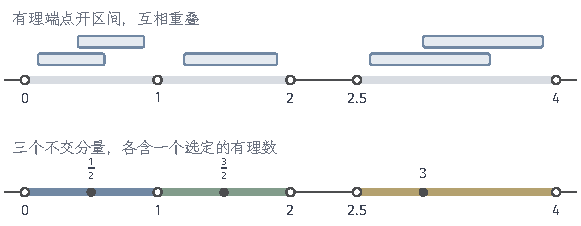
\includegraphics[width=98.4mm]{figures/02-abstract-mathematics/01-metric-and-measure/tikz/c2-open-set-components/figure.pdf}
  \caption{开集$U=(0,1)\cup(1,2)\cup(2.5,4)$的两种区间表示。上行：$U$中若干有理端点开区间，它们互相重叠，全体有理端点区间之并恰为$U$；下行：按“两点之间的闭区间是否含于$U$”分类得到三个互不相交的分量，每个分量中选一个有理数（圆点），说明分量至多可数。}
  \label{fig:measure-open-set-components}
\end{figure}

\paragraph{离散空间}
若$X$是有限集或可数集，并且每个单点都是闭集（例如带离散度量，或$\mathbb N$作为$\mathbb R$的子空间），那么任一子集$A$都是可数个闭单点的并，属于$\mathcal B(X)$，即$\mathcal B(X)=\mathcal P(X)$。在这类空间上，测量任意子集都不受限制，下面的计数测度和加权点测度直接以全部子集为可测范围。第~\ref{chap:integration}章将看到，离散空间上的积分就是加权求和，连续情形与离散情形由此纳入同一种形式。

\subsection{测度的定义}
\label{sec:measure-definition}

可测范围确定以后，需要给每个可测集合配一个非负的大小，并要求上一节提出的可数可加性成立。允许取值$+\infty$，是因为整条实轴的长度、无限集合的元素个数都没有有限的值。约定$[0,+\infty]$中$a+(+\infty)=+\infty$，非负项级数的和是部分和的上确界。

\begin{definition}[测度]
\label{def:measure-measure}
设$(X,\mathcal A)$是可测空间。映射$\mu:\mathcal A\to[0,+\infty]$若满足
\begin{enumerate}
 \item $\mu(\varnothing)=0$；
 \item 对两两不交的$A_1,A_2,\dots\in\mathcal A$，有$\mu\bigl(\bigcup_{n\ge1}A_n\bigr)=\sum_{n\ge1}\mu(A_n)$，
\end{enumerate}
则称$\mu$为$(X,\mathcal A)$上的\term{测度}（measure），称$(X,\mathcal A,\mu)$为\term{测度空间}（measure space）。第2条称为\term{可数可加性}（countable additivity）。
\end{definition}

\paragraph{计数测度、Dirac测度与加权点测度}
在任意可测空间上，令$\mu(A)=\#A$（$A$为无限集时取$+\infty$），称为\term{计数测度}（counting measure）。核对可数可加性：若不交的$A_n$中只有有限个非空且都为有限集，两边都是元素总数；若某个$A_n$无限，或有无限多个$A_n$非空，并集无限，右边的级数也发散到$+\infty$。

固定$x\in X$，令$\delta_x(A)=\mathbf 1_A(x)$，即$x\in A$时取$1$、否则取$0$，称为点$x$处的\term{Dirac测度}（Dirac measure）。不交集合列中至多一个含$x$，所以$\mathbf 1_{\bigcup_nA_n}(x)=\sum_n\mathbf 1_{A_n}(x)$，可数可加性成立。这个定义只读取可测集合$A$是否含$x$，并不要求单点$\{x\}$本身可测。例如在$\mathcal A=\{\varnothing,\{1,2\},\{3,4\},X\}$上，$\delta_1$给$\{1,2\}$赋值$1$、给$\{3,4\}$赋值$0$，尽管$\{1\}$不可测。

把有限个点质量按非负权重相加，得到$\mu=\sum_{k=1}^mw_k\delta_{x_k}$，即$\mu(A)=\sum_{k:x_k\in A}w_k$。它是第~\ref{sec:measure-counting-length}小节中加权计数的推广，可数可加性由每个$\delta_{x_k}$的可数可加性逐项相加得到。可数个点、可数个测度的加权和需要交换两重求和，留到第~\ref{sec:measure-properties}小节证明。

\paragraph{有限性条件}
测度可以在整体上取$+\infty$，但不同测度“无限”的方式差别很大。

\begin{definition}[有限测度、概率测度与$\sigma$有限测度]
\label{def:measure-finiteness}
设$(X,\mathcal A,\mu)$是测度空间。若$\mu(X)<+\infty$，称$\mu$为\term{有限测度}（finite measure）；若$\mu(X)=1$，称$\mu$为\term{概率测度}（probability measure）；若存在$X_1,X_2,\dots\in\mathcal A$使$X=\bigcup_nX_n$且每个$\mu(X_n)<+\infty$，称$\mu$为\term{$\sigma$有限测度}（sigma-finite measure）。
\end{definition}

有限测度都是$\sigma$有限的，取$X_1=X$即可。$\mathbb N$上的计数测度总量为$+\infty$，但$\mathbb N=\bigcup_n\{n\}$且每个单点计数为$1$，所以它$\sigma$有限：整体无限，却能切成可数个有限片。$\mathbb R$上以全部子集为可测范围的计数测度不是$\sigma$有限的：若$\mathbb R=\bigcup_nX_n$且每个$\#X_n<+\infty$，则$\mathbb R$是可数个有限集之并，从而可数，矛盾。后面一些结论（例如唯一性和分解定理）需要$\sigma$有限条件，一些结论（例如下一小节的基本性质）不需要；我们在每处单独声明，不把它当成统一假设。

\subsection{测度的性质}
\label{sec:measure-properties}

可数可加性只直接说到不交集合。比较两个有包含关系的集合、处理互相重叠的集合以及取集合列的极限，都要先把集合拆成不交的部分。

\begin{theorem}[测度的基本性质]
\label{thm:measure-basic-properties}
设$(X,\mathcal A,\mu)$是测度空间，以下集合都属于$\mathcal A$。
\begin{enumerate}
 \item 有限可加性：若$A_1,\dots,A_m$两两不交，则它们的并的测度等于各自测度之和，即$\mu(\bigcup_{k=1}^mA_k)=\sum_{k=1}^m\mu(A_k)$。
 \item 单调性：$A\subseteq B$蕴含$\mu(A)\le\mu(B)$；若还有$\mu(A)<+\infty$，则$\mu(B\setminus A)=\mu(B)-\mu(A)$。
 \item 可数次可加性：$\mu(\bigcup_nA_n)\le\sum_n\mu(A_n)$，其中$A_n$不必互不相交。
 \item 从下连续性：若$A_1\subseteq A_2\subseteq\cdots$，则$\mu(\bigcup_nA_n)=\lim_{n\to\infty}\mu(A_n)$。
 \item 从上连续性：若$A_1\supseteq A_2\supseteq\cdots$且$\mu(A_1)<+\infty$，则$\mu(\bigcap_nA_n)=\lim_{n\to\infty}\mu(A_n)$。
\end{enumerate}
\end{theorem}

\begin{proof}
第1条在可数可加性中令$A_n=\varnothing$（$n>m$）即得。对第2条，$B=A\cup(B\setminus A)$是不交并，由第1条$\mu(B)=\mu(A)+\mu(B\setminus A)\ge\mu(A)$；当$\mu(A)$有限时两边可以减去$\mu(A)$。

对第3条，令$B_1=A_1$，$B_n=A_n\setminus\bigcup_{k<n}A_k$。$B_n$两两不交，$B_n\subseteq A_n$，且$\bigcup_{k\le n}B_k=\bigcup_{k\le n}A_k$对每个$n$成立，从而$\bigcup_nB_n=\bigcup_nA_n$。由可数可加性与单调性，$\mu(\bigcup_nA_n)=\sum_n\mu(B_n)\le\sum_n\mu(A_n)$。

对第4条，令$A_0=\varnothing$，$D_n=A_n\setminus A_{n-1}$。相邻差集$D_n$两两不交，$A_n=\bigcup_{k\le n}D_k$，$\bigcup_nA_n=\bigcup_kD_k$，所以
\[
 \mu\Bigl(\bigcup_nA_n\Bigr)=\sum_{k=1}^{\infty}\mu(D_k)=\lim_{n\to\infty}\sum_{k=1}^n\mu(D_k)=\lim_{n\to\infty}\mu(A_n).
\]

对第5条，令$C_n=A_1\setminus A_n$，它们递增，并$\bigcup_nC_n=A_1\setminus\bigcap_nA_n$。由第4条，$\mu(A_1\setminus\bigcap_nA_n)=\lim_n\mu(A_1\setminus A_n)$。因为$\mu(A_1)<+\infty$，第2条允许两边写成差：$\mu(A_1)-\mu(\bigcap_nA_n)=\mu(A_1)-\lim_n\mu(A_n)$，消去有限数$\mu(A_1)$即得结论。
\end{proof}

第5条中的有限性条件不能省略。在$\mathbb N$上取计数测度与尾集$A_n=\{n,n+1,\dots\}$：每个$A_n$都是无限集，$\mu(A_n)=+\infty$，而$\bigcap_nA_n=\varnothing$，测度为$0$。证明在这里失效的位置是“两边减去$\mu(A_1)$”：$+\infty-+\infty$没有意义。只要从某项起$\mu(A_n)$有限，把这一项当作首项即可应用第5条。

\paragraph{限制与加权和}
从已有测度得到新测度，有三种常用操作，分别改变底集、可测范围与赋权规则。设$E\in\mathcal A$。令$\mu|_E(A)=\mu(A\cap E)$，$A\in\mathcal A$，它仍是$(X,\mathcal A)$上的测度，只把质量保留在$E$内；也可以把它看作迹$\sigma$代数$\mathcal A_E$上的测度，此时底集缩小为$E$。若$\mathcal G$是$\mathcal A$的子$\sigma$代数，把$\mu$只在$\mathcal G$上取值，得到$(X,\mathcal G)$上的测度$\mu|_{\mathcal G}$，底集与已有集合的取值都不变，只是可以询问的集合变少了。第三种操作把若干测度加权求和，需要先确认可数可加性在求和后保持。

\begin{lemma}[测度的可数加权和]
\label{lem:measure-weighted-sum}
设$\mu_1,\mu_2,\dots$是$(X,\mathcal A)$上的测度，$c_1,c_2,\dots\in[0,+\infty]$，约定$0\cdot(+\infty)=0$。则$\mu(A)=\sum_{k\ge1}c_k\mu_k(A)$定义$(X,\mathcal A)$上的测度。
\end{lemma}

\begin{proof}
$\mu(\varnothing)=0$是直接的。设$A_n$两两不交，记$a_{k,n}=c_k\mu_k(A_n)\in[0,+\infty]$。由各$\mu_k$的可数可加性，$\mu(\bigcup_nA_n)=\sum_k\sum_na_{k,n}$，而$\sum_n\mu(A_n)=\sum_n\sum_ka_{k,n}$，只需说明非负二重级数可以交换求和次序。对任意有限的$K,N$，有限和可以交换：$\sum_{k\le K}\sum_{n\le N}a_{k,n}=\sum_{n\le N}\sum_{k\le K}a_{k,n}\le\sum_n\sum_ka_{k,n}$。先令$N\to\infty$，再令$K\to\infty$，左边单调增加到$\sum_k\sum_na_{k,n}$，所以它不超过$\sum_n\sum_ka_{k,n}$；交换两者的角色得到反向不等式。约定$0\cdot(+\infty)=0$保证$c_k=0$的项对任何集合都贡献零，使上面的逐项计算不出现无定义的乘积。
\end{proof}

例如在$\mathbb N=\{1,2,\dots\}$上取$\mu=\sum_{n\ge1}2^{-n}\delta_n$，则$\mu(\mathbb N)=\sum_n2^{-n}=1$，$\mu$是概率测度；偶数集的测度为$\sum_{m\ge1}4^{-m}=1/3$，奇数集为$2/3$。可数个点的加权测度$\sum_kw_k\delta_{x_k}$也由引理~\ref{lem:measure-weighted-sum}成为测度。

\subsection{零测集}
\label{sec:measure-null-sets}

\paragraph{零测集与几乎处处}
测量中常有一些例外点：它们存在，但质量为零，不影响任何集合的大小。我们希望能说“除去一个可以忽略的集合，某性质成立”。

\begin{definition}[零测集与几乎处处]
\label{def:measure-null-set}
设$(X,\mathcal A,\mu)$是测度空间。满足$\mu(N)=0$的$N\in\mathcal A$称为$\mu$-\term{零测集}（null set）。若关于$X$中点的某个性质不成立的点全体包含于某个$\mu$-零测集，称该性质$\mu$-\term{几乎处处}（almost everywhere）成立，记作$\mu$-a.e.。
\end{definition}

定义只要求失败点集\emph{包含于}一个零测集，因为失败点集本身未必可测。“几乎处处”总是相对于当前测度而言的。在$X=\{0,1\}$与$\mathcal A=\mathcal P(X)$上，集合$\{1\}$是$\delta_0$的零测集，却承载$\delta_1$的全部质量；于是“函数在点$1$以外取零”对$\delta_0$几乎处处成立，对$\delta_1$不成立。

可数个零测例外可以合并：若$N_1,N_2,\dots$都是$\mu$-零测集，由可数次可加性，$\mu(\bigcup_nN_n)\le\sum_n\mu(N_n)=0$。因此一列性质若各自几乎处处成立，它们同时几乎处处成立。这一论证依赖可数次可加性，对不可数个零测集不适用；第~\ref{sec:measure-lebesgue}小节构造长度测度后会看到，$[0,1]$是不可数个长度为零的单点之并，自身长度却为$1$。

\paragraph{完备性与完备化}
零测集的子集“更应当”可以忽略，可是它不一定在$\mathcal A$中。在$X=\{1,2,3\}$上取$\mathcal A=\{\varnothing,\{1\},\{2,3\},X\}$与$\mu=\delta_1$，$\{2,3\}$是零测集，它的子集$\{2\}$却不可测，连“$\{2\}$的测度为零”这句话都无法说出。

\begin{definition}[完备测度空间]
\label{def:measure-complete}
若测度空间$(X,\mathcal A,\mu)$中每个$\mu$-零测集的每个子集都属于$\mathcal A$，称该测度空间是\term{完备}（complete）的。
\end{definition}

这里的完备与第~\ref{sec:metric-convergence-completeness}节度量空间的完备性（Cauchy列收敛）是两个不同概念，只是同名。不完备的测度空间可以通过补入零测集的子集加以修补。

\begin{theorem}[测度空间的完备化]
\label{thm:measure-completion}
设$(X,\mathcal A,\mu)$是测度空间。令$\overline{\mathcal A}$为形如$A\cup M$的集合全体，其中$A\in\mathcal A$，$M$包含于某个$\mu$-零测集；规定$\overline\mu(A\cup M)=\mu(A)$。则$\overline{\mathcal A}$是包含$\mathcal A$的$\sigma$代数，$\overline\mu$是其上不依赖表示方式的测度，在$\mathcal A$上与$\mu$一致，且$(X,\overline{\mathcal A},\overline\mu)$完备。它称为$(X,\mathcal A,\mu)$的\term{完备化}（completion）。
\end{theorem}

\begin{proof}
先证赋值与表示无关。设$A\cup M=A'\cup M'$，其中$M\subseteq N$、$M'\subseteq N'$，$N,N'$为零测集。则$A\subseteq A'\cup M'\subseteq A'\cup N'$，由单调性与次可加性$\mu(A)\le\mu(A')+\mu(N')=\mu(A')$；对称地$\mu(A')\le\mu(A)$。

再证$\overline{\mathcal A}$是$\sigma$代数。取$M=\varnothing$可知$\mathcal A\subseteq\overline{\mathcal A}$。对补集，设$M\subseteq N$，则
\[
 X\setminus(A\cup M)=\bigl((X\setminus A)\setminus N\bigr)\cup\bigl((X\setminus A)\cap(N\setminus M)\bigr),
\]
第一项属于$\mathcal A$，第二项包含于$N$。对可数并，$\bigcup_n(A_n\cup M_n)=(\bigcup_nA_n)\cup(\bigcup_nM_n)$，而$\bigcup_nM_n\subseteq\bigcup_nN_n$，后者是零测集。

然后证可数可加性。若$A_n\cup M_n$两两不交，则$A_n$两两不交，$\overline\mu(\bigcup_n(A_n\cup M_n))=\mu(\bigcup_nA_n)=\sum_n\mu(A_n)=\sum_n\overline\mu(A_n\cup M_n)$。最后证完备性：若$\overline\mu(A\cup M)=0$，则$\mu(A)=0$，$A\cup M\subseteq A\cup N$是$\mu$-零测集；它的任一子集$S$可写成$\varnothing\cup S$，属于$\overline{\mathcal A}$。
\end{proof}

在上面的例子中，零测集$\{2,3\}$的子集$\{2\}$、$\{3\}$被补入，$\overline{\mathcal A}=\mathcal P(X)$，并有$\overline\mu=\delta_1$。完备化不改变原有集合的测度，只把“包含于零测集”的集合也纳入可测范围并赋值为零。
